\documentclass{article}
\usepackage[utf8]{inputenc}
\usepackage{amssymb}
\usepackage{graphicx}
\usepackage{setspace}
\usepackage{listings}
\usepackage{float}
\usepackage{xcolor}
\usepackage{amsmath}
\usepackage{pgfplots}
\usepackage{subcaption}
\usepackage{hyperref}

\title{\textbf{High Performance Computer Architectures Practical Course \\ - Exercise 8 -} \\[10mm]}
\author{Tutorium 1 \\[10mm] David Jordan (6260776) \\[1mm] Florian Rüffer (7454628) \\[1mm] Michael Samjatin (7485765) \\[10mm]}


\lstset{
    language=C++,
    basicstyle=\ttfamily,
    keywordstyle=\color{blue},
    stringstyle=\color{red},
    commentstyle=\color{green},
    numbers=left,
    numberstyle=\normalsize,
    breaklines=true,
    showstringspaces=false,
    frame=single,
    linewidth=1\linewidth,
    captionpos=b
}
\renewcommand{\lstlistingname}{File}% Listing -> Algorithm
\renewcommand{\lstlistlistingname}{List of \lstlistingname s}% List of Listings -> List of Algorithms

\begin{document}
\maketitle
\newpage
\section*{1\_First}
\subsection*{Part 1}
In this part we have to compile and run the code for main1.cpp. The checkErr function is meant to check the return value of OpenCL function calls and returns an error message if one does occur.

\begin{lstlisting}[main1.cpp error function]
   checkErr(cl_int err, const char *name)
{
        // Error codes are indeed CL_SUCCESS == 0
        if (err != CL_SUCCESS)
        {
                std::cerr << "ERROR: " << name
                          << " (" << err << ")" << std::endl;
                exit(EXIT_FAILURE);
        }
}
\end{lstlisting}
We proceed to vary the sizes of the LIST\_SIZE variable. Upon running the program we see that the program provides all permutations of adding together two integers to get the specified LIST\_SIZE. To summarize the functioning of the program:
After the program creates respective OpenCL context, command queue and memory buffer for each vector, it copies A and B into their respective memory buffers. It creates a program from the kernel source and then builds the program. It then creates the OpenCL kernel and executes it on the LIST:
\begin{lstlisting}[main1.cpp error function]
 size_t global_item_size = LIST_SIZE; // Process the entire lists
        size_t local_item_size = 1;          // Process in groups of 1

        ret = clEnqueueNDRangeKernel(command_queue, kernel, 1, NULL,
                                     &global_item_size, &local_item_size, 0, NULL, NULL);
        checkErr(ret, "clEnqueueNDRangeKernel");
\end{lstlisting}

It stores the memory buffer C on the device to the local variable C and displays the result of the addition on the console.

\begin{figure}[H]
    \centering
    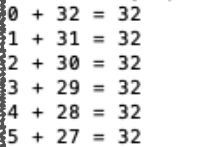
\includegraphics[scale=0.6]{opencl_1.png} 
    \caption{console output}
    \label{fig:graph}
\end{figure}

\subsection*{Part 2}
The following lines retrieve the build log information for the program compilation:
\begin{lstlisting}[getting build log]
 char* build_log; // the pointer to a char  
                  //array that will store the build log information
    size_t log_size;
    // First call to know the proper size
    clGetProgramBuildInfo(program, device_id, CL_PROGRAM_BUILD_LOG, 0, NULL, &log_size);
    build_log = new char[log_size+1];
    // Second call to get the log
    clGetProgramBuildInfo(program, device_id, CL_PROGRAM_BUILD_LOG, log_size, build_log, NULL);
    build_log[log_size] = '\0';
    cout << build_log << endl;
    delete[] build_log;
\end{lstlisting}
In order to have a comparison for the runtimes  of the OpenCL Code, a normal scalar version of addition in C++ is implemented:

\begin{lstlisting}[scalar add in cpp]
typedef float DataType;

void scalar_add( DataType A,  DataType B,  DataType C) {

      // Do the operation
    C = A + B;
}
\end{lstlisting}
This function is then later called together with a timing function. 
Upon executing the program with the simple addition, the scalar version turns out to be almost two orders of magnitude faster in the execution of this simple operation:
\begin{figure}[H]
    \centering
    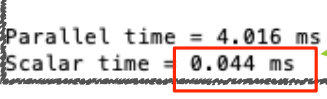
\includegraphics[scale=0.6]{scalar_add.png} 
    \caption{scalar addition is much faster}
    \label{fig:graph}
\end{figure}

This can only be because of significant overhead in OpenCL compared to the standard C++ version. 

Only when the complexity of the calculations is increased using expensive operations like sqrt and log() can the advantage of the OpenCL parallelisation come through. A sufficiently complicated calculation yields a threefold improvement of the Scalar time: 

\begin{figure}[H]
    \centering
    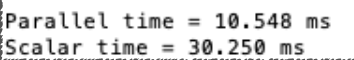
\includegraphics[scale=0.6]{logs_andsqrt.png} 
    \caption{for complex logs and sqrt times, parallel is much faster}
    \label{fig:graph}
\end{figure}

This can only be because these more complicated operations offer the opportunity to be parallellized by OpenCL, that is parts of these operations, where there are no data dependencies are executed simultaneously.

\subsection*{Part 3}
In this part we need to SIMDize the program. \\
We start off by creating the vector\_add\_kernel2.cl file,
which contains code to utilize SIMD capabilities.

\begin{lstlisting}[caption=vector\_add\_kernel2.cl]
    __kernel void vector_add(__global float *A, __global float *B, __global float *C) {
    
    
    int i = get_global_id(0);

    
    float4 a = vload4(i, A);
    float4 b = vload4(i, B);

    
    vstore4( a + b, i, C );
}
\end{lstlisting}
\noindent The first line defines a kernel function, which can be executed on an OpenCL device. \\
The function takes three parameters (A, B, C), which can be located in the global memory space.
Furthermore line 4 gets the id is of the current work item and assigns the i-th group of A, B and C to it.
In this case A, B and C are vectors with 4 elements each (line 7,8). \\
Finally line 11 stores the computed values into the $4 \cdot i$ element. \\
\newpage
\noindent Subsequently we will add / load this kernel to our code in the main.cpp file.

\begin{lstlisting}[caption=main.cpp]
#ifdef SIMD
    fp = fopen("vector_add_kernel2.cl", "r");
#else
    fp = fopen("vector_add_kernel.cl", "r");
#endif
    if (!fp) {
        fprintf(stderr, "Failed to load kernel.\n");
        exit(1);
    }
\end{lstlisting}

\noindent This part of the code add the new kernel to the main.cpp code base.
If it is available it will be used, if not another kernel (w/o SIMD) will be used.
If both of the cases above fail, we raise an error. \\\\

\noindent We also should not forget to add the preprocessing macro at the beginning of our code.
This allows us to use SIMD in commands, such as \#ifdef, to switch between scalar or simd execution during compile time.

\begin{lstlisting}[caption=main.cpp]
    #define SIMD
\end{lstlisting}

\noindent Adjust our list size, to be divisible by 4.
\begin{lstlisting}[caption=main.cpp]
    const int LIST_SIZE = 1024;
\end{lstlisting}

\noindent Last but not least, we need to compute the item size.
We do this the same way, in which we have loaded the kernel.

\begin{lstlisting}[caption=main.cpp]
    #ifdef SIMD
    size_t global_item_size = LIST_SIZE/4; // Process the entire lists
#else
    size_t global_item_size = LIST_SIZE;
#endif
    size_t local_item_size = 64; // Process in groups of 64
\end{lstlisting}

\noindent If we have defined SIMD, we will determine the number of work items we need.
For our list size this would result in 256 work items.
If we SIMD is not defined our item size will equal the list size.
Lastly if both of the cases above fail to trigger, we will process in groups of 64.

\subsection*{Part 4}
In this part sub devices are added. \\
Starting off by gathering device information:
\begin{lstlisting}
    cl_platform_id platform_id = NULL;
    cl_device_id device_id = NULL;   
    cl_uint ret_num_devices;
    cl_uint ret_num_platforms;
    cl_int ret = clGetPlatformIDs(1, &platform_id, &ret_num_platforms);
    checkErr(ret, "clGetPlatformIDs");
\end{lstlisting}
The first two lines initialize as NULL and will be used later on to refer the platform and device.
The next two lines hold the number of platforms and devices.
Line 5 denotes an error code (cl\_int), which tells if the platform id was fetched successfully.
Here only one platform is returned and written to platform\_id, due to the first parameter. Also an error check is performed.\\\\

\noindent Here we perform the same task as described above, but for our device.\\
CL\_DEVICE\_TYPE\_CPU restricts us to devices of a certain type.
\begin{lstlisting}
    ret = clGetDeviceIDs( platform_id, CL_DEVICE_TYPE_CPU, 1, 
    &device_id, &ret_num_devices);
    checkErr(ret, "clGetDeviceIDs");
\end{lstlisting}

\noindent These two lines denote variables to hold the number and id of the created subdevices.
\begin{lstlisting}
    cl_uint num_devices_ret;
    cl_device_id  out_devices[80];
\end{lstlisting}

\noindent This part denotes the properties based on which the device will be partitioned into subdevices.
An equal partion means dividing it into as many parts as possible, while each part contains the same number of compute units (in this case 2).
Subsequently the devices are created based on the defined properties.
At the end again an error check is performed.
\begin{lstlisting}
    const cl_device_partition_property props[] = {CL_DEVICE_PARTITION_EQUALLY, 2, 0};
    ret = clCreateSubDevices ( device_id, props, 80 , out_devices , &num_devices_ret );
    checkErr(ret, "clCreateSubDevices");
\end{lstlisting}
\newpage

The other partition methods, include partitioning by counts and affinity domain.
When we partition by count, we can specify the exact number of compute units each subdevice should have.
This allows a more find-grained control.
\begin{lstlisting}
    const cl_device_partition_property props[] = {CL_DEVICE_PARTITION_BY_COUNTS, 1, 1, CL_DEVICE_PARTITION_BY_COUNTS_LIST_END, 0};
\end{lstlisting}
Additionally there is the partitioning method by affinity domain.
Those affinity domains are specific areas of the device (e.g. L1, L2 Cache).
The subdevices will then be created and have an affinity to a certain affinity domain.
The code below will result in an affinity (e.g. faster access) to the L1 Cache.
\begin{lstlisting}
    const cl_device_partition_property props[] = {CL_DEVICE_PARTITION_BY_AFFINITY_DOMAIN, CL_DEVICE_AFFINITY_DOMAIN_L1_CACHE, 0};
\end{lstlisting}
\subsection*{Part 5}
\subsection*{Part 6}
\subsection*{Appendix}

\begin{lstlisting}[caption=example code]
    #pragma omp parallel for num_threads(omp_get_num_procs())
\end{lstlisting}

\begin{figure}[H]
    \centering
    \includegraphics[scale=0.6]{example-image.png} 
    \caption{example image}
    \label{fig:graph}
\end{figure}



\end{document}